
% Homework template for MA 614, Spring 2011.  When a line begins with the percent sign, the typesetter ignores it.  So, use percent signs at the beginning of lines to insert comments to yourself.


% Set the document class.  The command [11pt] sets the font at 11 point, which is nicer to read.  The default would be 10pt
\documentclass[11pt]{amsart} 


% Call packages that allow you to invoke certain mathematical symbols.
\usepackage{amssymb,amsmath,amsthm}
\usepackage[framed,numbered,autolinebreaks,useliterate]{mcode}
\usepackage{natbib}
\usepackage{hyperref}
\usepackage{float}
%\bibpunct{(}{)}{;}{a}{,}{,}
\usepackage{graphicx}
% Set the title, author, and date information.
\title{Homework 1: Graphical methods for high dimensional data in statistics }

\author{Anil A. Aksu }
\date{\today}


% Formally begin the document and make the title.
\begin{document}

\maketitle
 2-D and 3-D random data are generated by using built-in functions of $R$ programming language and Car data is obtained by using $car$ library in $R$. The particular script is given in Appendix \ref{Rcodes}. In this homework, the graphical methods given by \cite{Grinstein2001} are used. These are Heat Map, 3-D scatter plot and Matrix of scatter plots. 
\section*{\bf{Heat Map}}
\begin{figure}[H]
\centering
 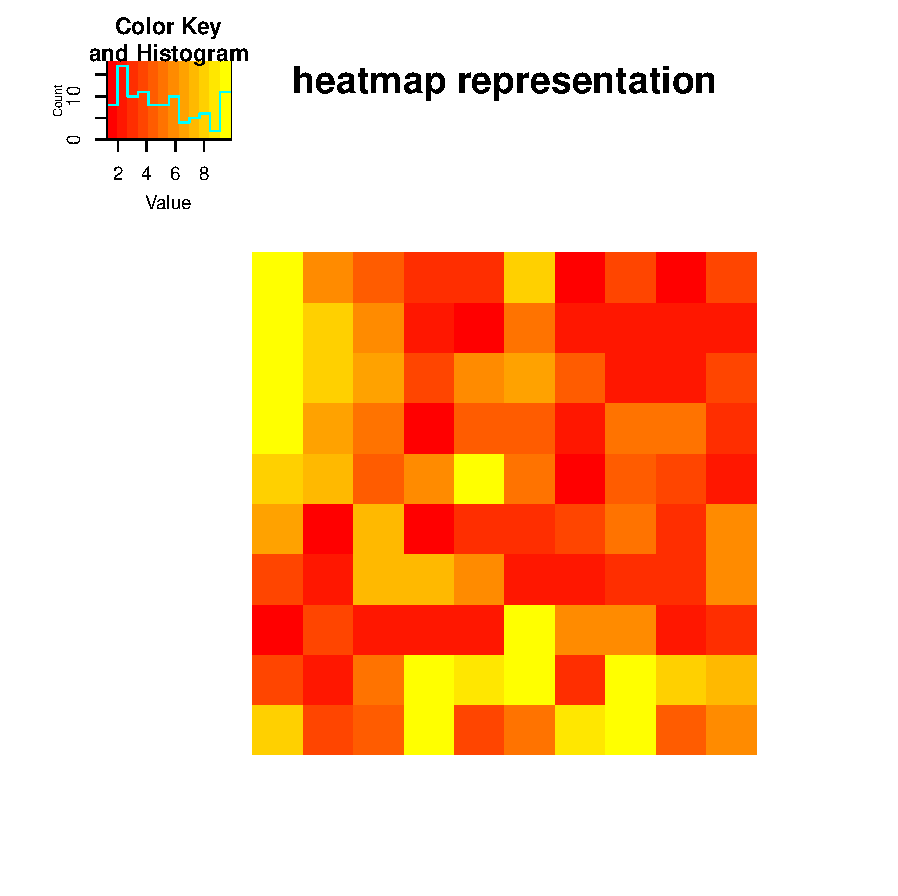
\includegraphics[scale=0.7]{Heatmap}% Images in 100% size
  \caption{Heap map of random data set. }
\label{fig:Heatmap}
\end{figure} 

\newpage

 \section*{\bf{3-D Scatter Plot }}
 \begin{figure}[H]
\centering
 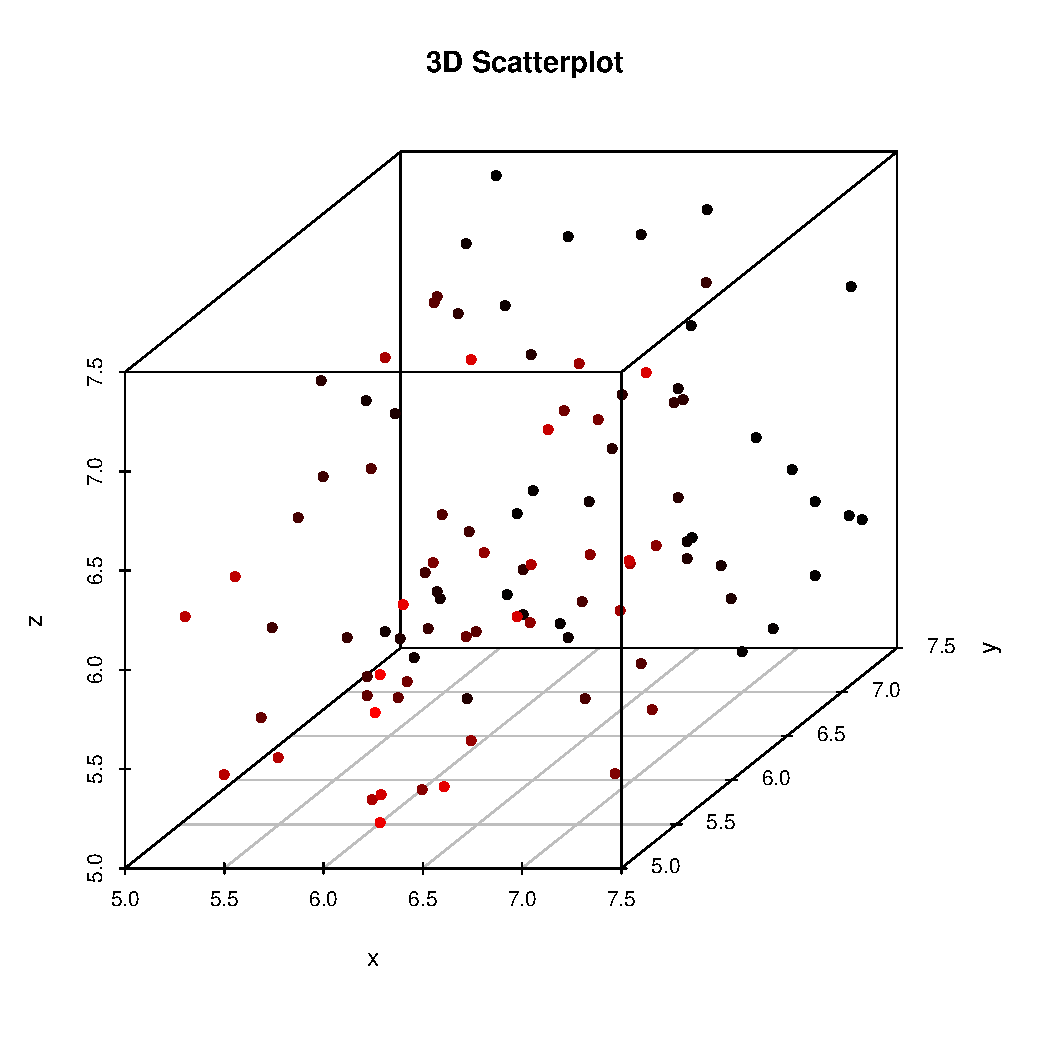
\includegraphics[scale=0.7]{scatter3D}% Images in 100% size
  \caption{3-D of Scatter Plot. }
\label{fig:ScatterMat}
\end{figure} 
\newpage

\section*{\bf{Matrix of Scatter plots}}

\begin{figure}[H]
\centering
 \includegraphics[scale=0.7]{ScatterMatrix}% Images in 100% size
  \caption{Matrix of Scatter plots. }
\label{fig:ScatterMat}
\end{figure} 

\appendix

\section{R Codes \label{Rcodes}}
\lstinputlisting{HighDimData.R} 

\bibliographystyle{plainnat}
% Note the spaces between the initials
\bibliography{Bayes}
\end{document}
